\documentclass[
  captions=tableheading,
  bibliography=totoc, 
  titepage=firstiscover,
]{scrartcl}

\usepackage{blindtext} %neuer input

\usepackage{longtable} % Tabellen über mehrere Seiten

\usepackage[utf8]{inputenc} %neuer input

\usepackage{scrhack}

\usepackage[aux]{rerunfilecheck} %Warnung falls nochmal kompiliert werden muss

\usepackage{fontspec} %Fonteinstellungen

\recalctypearea{}

\usepackage[main=ngerman]{babel} %deutsche Spracheinstellung

\usepackage{ragged2e} %neuer input

\usepackage{amsmath, nccmath}

\usepackage{amssymb} %viele mathe Symbole

\usepackage{mathtools} %Erweiterungen für amsmath


\DeclarePairedDelimiter{\abs}{\lvert}{\rvert}
\DeclarePairedDelimiter{\norm}{\lVert}{\rVert}

\DeclarePairedDelimiter{\bra}{\langle}{\rvert}
\DeclarePairedDelimiter{\ket}{\lvert}{\rangle}

\DeclarePairedDelimiterX{\braket}[2]{\langle}{\rangle}{
#1 \delimsize| #2
}

\NewDocumentCommand \dif {m}
{
\mathinner{\symup{d} #1}
}


\usepackage[
  math-style=ISO,
  bold-style=ISO,
  sans-style=italic,
  nabla=upright,
  partial=upright,
  warnings-off={
    mathtools-colon,
    mathtools-overbracket,
  },
]{unicode-math}

\setmathfont{Latin Modern Math}
\setmathfont{XITS Math}[range={scr, bfscr}]
\setmathfont{XITS Math}[range={cal, bfcal}, StylisticSet=1]


\usepackage[
  locale=DE,
  separate-uncertainty=true,
  per-mode=reciprocal,
  output-decimal-marker={,},
]{siunitx}

\usepackage[autostyle]{csquotes} %richtige Anführungszeichen

\usepackage{xfrac}

\usepackage{float}

\floatplacement{figure}{htbp}

\floatplacement{table}{htbp}

\usepackage[ %floats innerhalb einer section halten
  section,   %floats innerhalb er section halten
  below,     %unterhalb der Section aber auf der selben Seite ist ok
]{placeins}

\usepackage[
  labelfont=bf,
  font=small,
  width=0.9\textwidth,
]{caption}

\usepackage{subcaption} %subfigure, subtable, subref

\usepackage{graphicx}

\usepackage{grffile}

\usepackage{booktabs}

\usepackage{microtype} %Verbesserungen am Schriftbild

\usepackage[
backend=biber,
]{biblatex}

\addbibresource{../lit.bib}

\usepackage[ %Hyperlinks im Dokument
  german,
  unicode,
  pdfusetitle,
  pdfcreator={},
  pdfproducer={},
]{hyperref}

\usepackage{bookmark}

\usepackage[shortcuts]{extdash}

%\usepackage{warpcol}


\begin{document}
    \title{V203 Verdampfungswärme}
    \author{  
    Tobias Rücker\\
    \texorpdfstring{\href{mailto:tobias.ruecker@tu-dortmund.de}{tobias.ruecker@tu-dortmund.de}
    \and}{,} 
    Paul Störbrock\\
    \texorpdfstring{\href{mailto:paul.stoerbrock@tu-dortmund.de}{paul.stoerbrock@tu-dortmund.de}}{}
    }
    \date{Durchführung: 17.12.2019, Abgabe: 07.01.2020\vspace{-4ex}}
\maketitle
\center{\Large Versuchsgruppe: \textbf{42}}
    
    \begin{abstract}
    \centering
        \textbf{Ziel:} 
    \end{abstract}

\newpage
\tableofcontents
\newpage

% Theorie %%%%%%%%%%%%%%%%%%%%%%%%%%%%%%%%%%%%%%%%%%%%%%%%%%%%%%%%%%%%%%%%%%%%%%%%%%%%%%%%%%%%%%%%%%%%%%%%%%%%%%%%%%%%%%%%%%%%%%%%%%%%%%%%%%%%%%%%%%%%%%%%%%%%%%%%%%%%%%%%%%%%%%%%%%%%%%%%%%%%%%%%%%%%%%%%%%

\section{Theorie}

% Versuchsaufbau + Versuchsdurchführung %%%%%%%%%%%%%%%%%%%%%%%%%%%%%%%%%%%%%%%%%%%%%%%%%%%%%%%%%%%%%%%%%%%%%%%%%%%%%%%%%%%%%%%%%%%%%%%%%%%%%%%%%%%%%%%%%%%%%%%%%%%%%%%%%%%%%%%%%%%%%%%%%%%%%%%%%%%%%%%%%%%%%%%%%%%%%%%%%%%%%%%%%%%%%%%%%%

% unter 1 bar ----------------------------------------------------------------------------------------------------------------------------------------------------------------------------------------------------------------------------------

\section{Versuchsaufbau und Versuchsdurchführung}\justifying

\flushleft{Aufbau\;}\justifying und Durchführung für den Druckbereich unter $\SI{1}{\bar}$:

\flushleft{Benötigt\;}\justifying werden: \textit{Eine Wasserstrahlpumpe, ein Absperrhahn, eine Woulffsche Flasche, ein Belüftungsventil, ein Drosselventil, ein Manometer, 
einen Rückflußkühler, zwei Flüssigkeitsthermometer, einen Mehrhalskolben, eine regelbare Heizhaube und destilliertes und entgastes Wasser.}

\flushleft{Für\;}\justifying die Temperatur- und Druckermittelung unter $\SI{1}{\bar}$ wird der Versuch, wie in Abbildung \ref{fig:1} dargestellt,
aufgebaut.

\begin{figure}
    \centering
    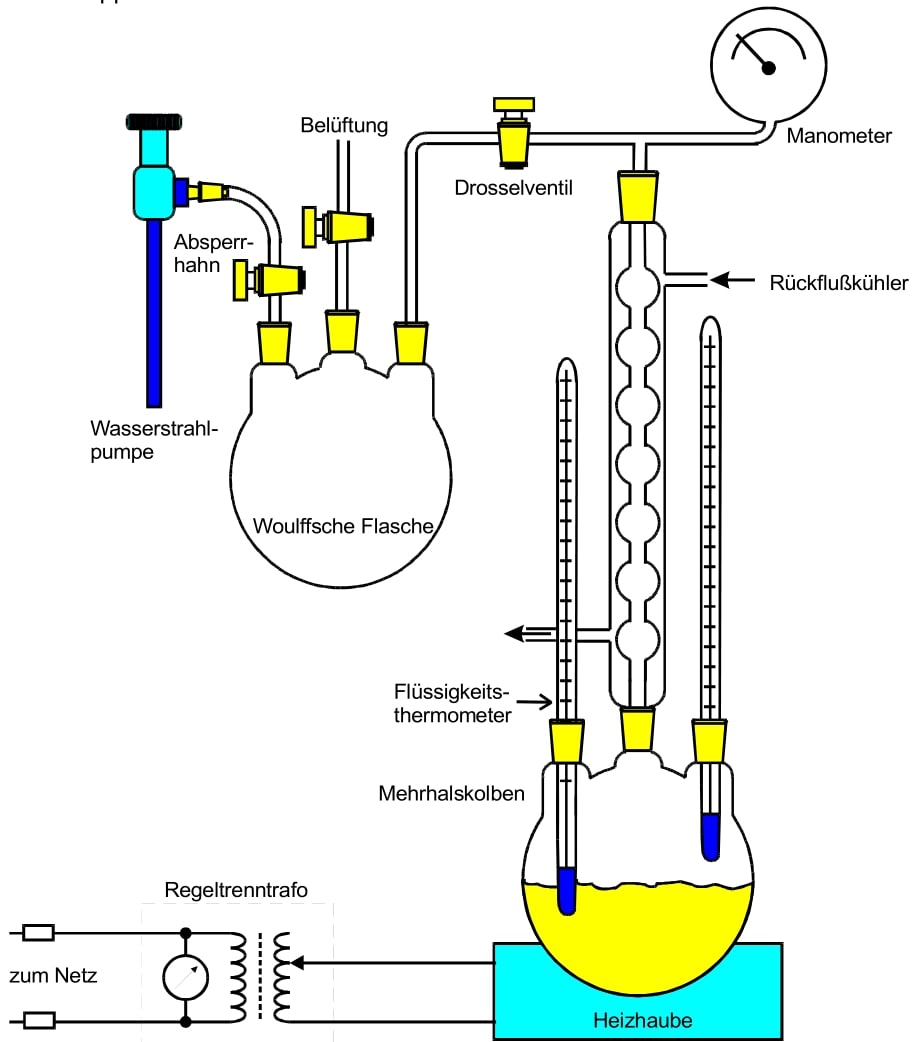
\includegraphics[width=0.75\linewidth]{./images/k1bar.jpg}
    \caption{Versuchsaufbau für Druckbereich $\leq \SI{1}{\bar}$ \cite{V203}}
    \label{fig:1}
\end{figure}
\newpage

\flushleft{Zu\;}\justifying Beginn muss der Mehrhalskolben evakuiert werden. Dazu wird das Belüftungsventil geschlossen und der Absperrhahn und
das Drosselventil geöffnet. Anschließend wird die Wasserstrahlpumpe eingeschaltet. Nun wird der interne Druck des Aufbaus mit dem Manometer
beobachtet bis der Druck auf ca. $\SI{60}{\milli\bar}$ gesunken ist. Ist dies eingetreten, wird das Drosselventil geschlossen, die Heizhaube
eingeschaltet und Wasser durch den Rückflußkühler geleitet. Gleichzeitig wird außerdem die Wasserstrahlpumpe abgeschaltet. Mit dem rechten
Thermometer wird nun die Temperatur des Gases gemessen. Hier misst das Gas eine Zimmertemperatur von $\SI{21}{\celsius}$. Es wird für jeden 
weiteren $\SI{}{\celsius}$ der entsprechende Druck dem Manometer entnommen. Dieser Prozess wird wiederholt, bis in dem Mehrhalskolben ein Druck 
von $\SI{1}{\bar}$ ($\SI{1000}{\milli\bar}$) herrscht. Abschließend wird die Heizhaube ausgeschaltet und alle Ventile geöffnet.  

% über 1 bar ----------------------------------------------------------------------------------------------------------------------------------------------------------------------------------------------------------------------------------

\flushleft{Aufbau\;}\justifying und Durchführung für den Druckbereich über $\SI{1}{\bar}$:

\flushleft{Benötigt\;}\justifying werden: \textit{Ein Flüssigkeitsthermometer, ein Drucksensor, ein analoges Manometer, ein U-Rohr, ein Metallzylinder, eine Heizwicklung 
(hier ein elektrischer Heizkörper).}

\flushleft{Für\;}\justifying die Temperatur- und Druckermittelung über $\SI{1}{\bar}$, wird der Versuch ähnlich zur Abbildung \ref{fig:2} aufgebaut. 
Hier wird allerdings die Kühlschale weggelassen und die Heizwicklung durch einen, unter den Zylinder befindlichen, Heizkörper ersetzt. 

\begin{figure}
    \centering
    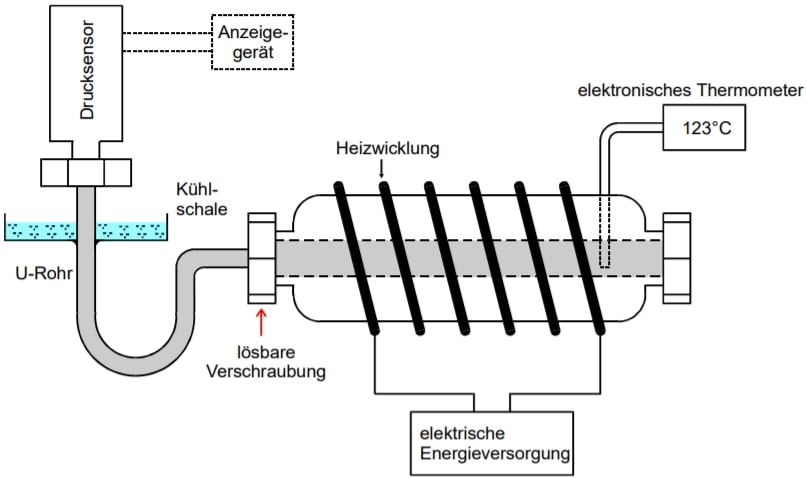
\includegraphics[width=\linewidth]{./images/g1bar.jpg}
    \caption{Versuchsaufbau für Druckbereich $\geq \SI{1}{\bar}$ \cite{V203}}
    \label{fig:1}
\end{figure}

\flushleft{Zuerst\;}\justifying wird der Heizkörper eingeschaltet. Anschließend wird die Temperatur für jeden halben $\SI{}{\bar}$ vom Thermometer
abgelesen. Dies wird wiederholt, bis das Manometer $\SI{15}{\bar}$ anzeigt. Abschließend wird der Heizkörper ausgeschaltet.

% Auswertung %%%%%%%%%%%%%%%%%%%%%%%%%%%%%%%%%%%%%%%%%%%%%%%%%%%%%%%%%%%%%%%%%%%%%%%%%%%%%%%%%%%%%%%%%%%%%%%%%%%%%%%%%%%%%%%%%%%%%%%%%%%%%%%%%%%%%%%%%%%%%%%%%%%%%%%%%%%%%%%%%%%%%%%%%%%%%%%%%%%%%%%%%%%%%%%%%%

\section{Auswertung}



\begin{table}
    \centering
    \input{table_k1bar.tex}
    \caption{Temperatur für Druck < 1bar}
    \label{tab:1}
\end{table}



\begin{table}
    \centering
    \input{table_g1bar.tex}
    \caption{Temperatur für Druck > 1bar}
    \label{tab:2}
\end{table}

% Diskussion %%%%%%%%%%%%%%%%%%%%%%%%%%%%%%%%%%%%%%%%%%%%%%%%%%%%%%%%%%%%%%%%%%%%%%%%%%%%%%%%%%%%%%%%%%%%%%%%%%%%%%%%%%%%%%%%%%%%%%%%%%%%%%%%%%%%%%%%%%%%%%%%%%%%%%%%%%%%%%%%%%%%%%%%%%%%%%%%%%%%%%%%%%%%%%%%%%

\section{Diskussion}

% Literatur %%%%%%%%%%%%%%%%%%%%%%%%%%%%%%%%%%%%%%%%%%%%%%%%%%%%%%%%%%%%%%%%%%%%%%%%%%%%%%%%%%%%%%%%%%%%%%%%%%%%%%%%%%%%%%%%%%%%%%%%%%%%%%%%%%%%%%%%%%%%%%%%%%%%%%%%%%%%%%%%%%%%%%%%%%%%%%%%%%%%%%%%%%%%%%%%%%

\newpage
\printbibliography

\end{document}
